\chapter{연구 결과 분석 및 평가}
\section{실험 환경과 평가 방법}
평가는 소프트웨어 구성, 좌표·센서 측정, 단일 블록 실기 동작, 전체 미션의 관찰을 구분하여 수행하였다. 본 장은 최종 CV+IK 경로의 자료를 중심으로 하며, 3장에 제시한 ACT의 58\%를 최종 시스템의 평가값으로 사용하지 않는다. 각 실험에서 확인한 범위와 남은 조건을 결과와 함께 제시한다.

9월 8일 기록에는 카메라 재고정과 단축 드리프트 검사, 아홉 점 캘리브레이션, 1차 미션의 외부 시간 제한 시험, 노란 블록의 위치 변경 후 파지·운반 관찰이 포함되어 있다. 시험 중 기본 설정을 변경하거나 실행 인자로 덮어쓴 항목이 있으므로, 저장소의 최신 YAML만으로 당시 실행을 재구성하지 않는다. 특히 배치 슬롯 보정과 모션 주파수를 구분하였다.

\begin{longtable}{@{}L{0.18\linewidth}L{0.32\linewidth}L{0.40\linewidth}@{}}
\caption{평가 단위와 성공 판단의 구분}\label{tab:eval-definitions}\\
\toprule 평가 단위 & 판단 대상 & 필요한 근거 \\\midrule
\endfirsthead
\toprule 평가 단위 & 판단 대상 & 필요한 근거 \\\midrule
\endhead
블록 검출 & 실제 블록의 검출·누락·오검출 & 정답이 표시된 프레임과 검출 결과. 현재 집계 추가 필요 \\
좌표 변환 & 대응점과 예측 위치의 차이 & 적합 잔차, LOO, 대응점 및 캘리브레이션 조건 \\
단일 파지 & 물체를 물고 들어 올렸는가 & 그리퍼 위치·부하, 단계 사진과 관찰 \\
단일 배치 & 목표 영역에 내려놓았는가 & 해제 전후 영상, 실제 경계와 블록 상태 \\
1차 전체 & 180초 내 다섯 블록 배치 & 시작 배치, 종료 시각과 다섯 블록의 실제 위치 \\
2차 전체 & 300초 내 적재와 5초 유지 & 적재 블록 수, 해제 이후 연속 영상과 유지시간 \\
소프트웨어 & 계약·상태 흐름·계산의 동작 & 단위·통합 테스트 기록. 실기 성능과 별도 평가 \\
\bottomrule
\end{longtable}

파지 부하값은 힘 단위로 교정되지 않았고, FK 좌표는 측정 관절값을 URDF로 변환한 값이다. 따라서 부하 500을 특정 파지력으로 환산하거나, FK 목표 오차를 물체와 턱의 실제 거리 오차로 표현하지 않는다. 다음 절의 수치는 이 정의에 따라 해석한다.

\section{캘리브레이션과 위치 오차 분석}
\subsection{아홉 점 적합 결과}
9월 8일 채택된 캘리브레이션의 대응점은 아홉 개이다. 첫 번째 점은 재시도한 \texttt{P1\_retry2}를 사용하였고 나머지는 P2--P9이다. 적합 보고서의 RMS는 8.18\,mm, 최대 잔차는 14.51\,mm, 최대 LOO 오차는 26.64\,mm이다. 적합기의 기준인 RMS 5\,mm 미만과 최대 LOO 8\,mm 미만을 모두 만족하지 못하였다.

\begin{table}[htbp]
\centering
\caption{9월 8일 채택한 아홉 점의 적합 잔차와 LOO 오차}\label{tab:calibration}
\begin{tabular}{@{}lrr@{}}
\toprule 대응점 & 적합 잔차 (mm) & LOO 오차 (mm) \\
\midrule
P1 (retry2) & 6.05 & 26.64 \\
P2 & 6.05 & 17.54 \\
P3 & 4.66 & 7.64 \\
P4 & 14.51 & 21.04 \\
P5 & 4.83 & 7.17 \\
P6 & 8.44 & 20.13 \\
P7 & 5.12 & 7.58 \\
P8 & 12.34 & 16.44 \\
P9 & 4.82 & 17.08 \\
\midrule
최대 & 14.51 & 26.64 \\
\bottomrule
\end{tabular}
\end{table}

\begin{figure}[htbp]
\centering
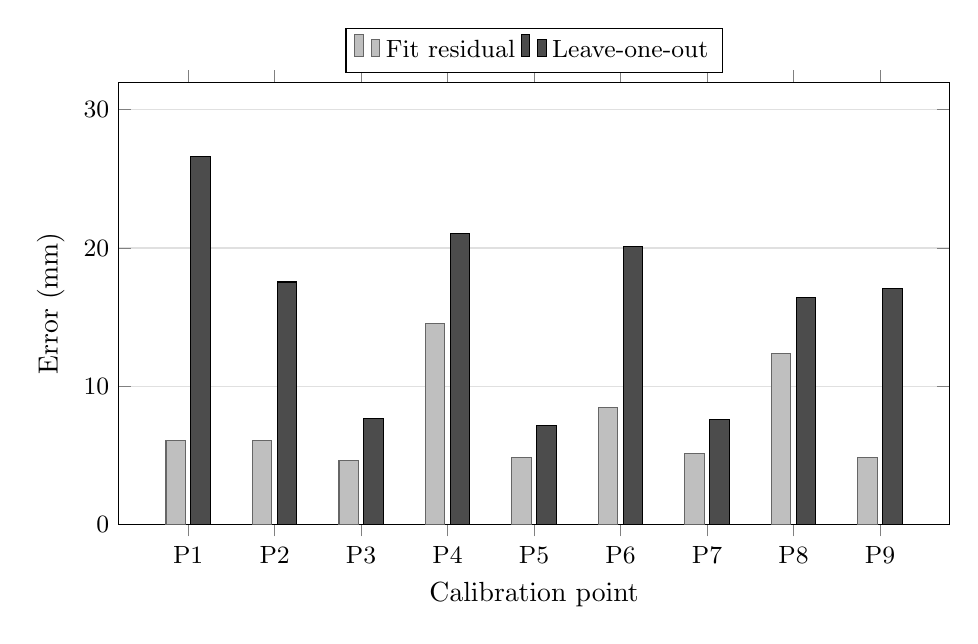
\begin{tikzpicture}
\begin{axis}[width=\linewidth,height=7.2cm,ybar,bar width=7pt,
symbolic x coords={P1,P2,P3,P4,P5,P6,P7,P8,P9},xtick=data,
ymin=0,ymax=32,ylabel={Error (mm)},xlabel={Calibration point},
legend style={at={(0.5,1.02)},anchor=south,legend columns=2,font=\small},
ymajorgrids=true,grid style={black!12},tick label style={font=\small}]
\addplot[fill=black!25,draw=black!60] coordinates {(P1,6.05)(P2,6.05)(P3,4.66)(P4,14.51)(P5,4.83)(P6,8.44)(P7,5.12)(P8,12.34)(P9,4.82)};
\addplot[fill=black!70,draw=black] coordinates {(P1,26.64)(P2,17.54)(P3,7.64)(P4,21.04)(P5,7.17)(P6,20.13)(P7,7.58)(P8,16.44)(P9,17.08)};
\legend{Fit residual,Leave-one-out}
\end{axis}
\end{tikzpicture}
\caption{표~\ref{tab:calibration}의 오차 비교. P1은 재시도 점이다. 적합에 사용한 점의 잔차보다 LOO 오차가 크게 나타나는 점이 있어 새 위치에 대한 정확도를 별도로 확인해야 한다.}
\label{fig:fit}
\end{figure}

이 결과는 사용한 변환이 시험에 투입되었다는 사실을 보여주지만 품질 기준 통과를 뜻하지 않는다. 일부 점의 잔차가 작더라도 모든 위치에서 그 정도의 정확도를 기대할 수 없으며, 최대 LOO 오차는 블록 폭 40\,mm에 비해 작은 값이라고 보기 어렵다. 대응점을 추가하거나 제외할 때에는 적합 RMS 감소만으로 변경을 채택하지 않고, 별도 위치에서의 물리적 파지 결과와 함께 확인해야 한다.

같은 적합 보고서에 기록된 파지 높이는 평균 16.2\,mm, 표준편차 6.8\,mm, 범위 1.2--26.3\,mm이다. 이는 로봇 베이스 프레임에서 기록한 높이이며 테이블로부터 블록 높이 20\,mm와 동일한 값이 아니다. 높이와 자세의 일관성이 충분히 확보되었는지, FK 기준점이 실제 턱의 어느 지점에 대응하는지 추가 검토할 필요가 있다.

\subsection{카메라 드리프트의 단축 검사}
보관된 두 드리프트 CSV는 각각 약 60.5초 동안 12개 표본을 기록하였다. 각 표본의 p95는 그 시점에서 대응된 코너 변위의 95백분위값이다. 첫 기록에서 표본별 p95의 최댓값은 2.775\,pixel이었고, 재검사 기록에서는 0.514\,pixel이었다. 재검사 값은 세션 요약의 약 0.51\,pixel과 대응한다.

\begin{figure}[htbp]
\centering
\begin{tikzpicture}
\begin{axis}[width=\linewidth,height=6.8cm,xlabel={Elapsed time (s)},ylabel={Frame-wise p95 drift (px)},
xmin=0,xmax=65,ymin=0,ymax=3.2,grid=major,grid style={black!12},
legend style={font=\small,at={(0.5,1.02)},anchor=south,legend columns=3},
tick label style={font=\small}]
\addplot[black!70,mark=square*,thick] table[x=elapsed_s,y=p95_px,col sep=comma]{figures/drift_initial.csv};
\addplot[black,mark=*,thick] table[x=elapsed_s,y=p95_px,col sep=comma]{figures/drift_retry.csv};
\addplot[dashed,black,domain=0:65,samples=2] {2};
\legend{Initial,Retry,2 px reference}
\end{axis}
\end{tikzpicture}
\caption{보관된 단축 드리프트 검사의 표본별 p95. 두 기록은 각각 별도 검사의 경과시간을 나타내며 10분 검사를 수행한 결과가 아니다.}
\label{fig:drift}
\end{figure}

재검사에서 개별 코너의 최대 변위는 12.354\,pixel까지 기록되어 p95보다 훨씬 컸다. 이는 일부 대응 코너의 변동이 전체적인 변위와 다를 수 있음을 보여주므로, 최대값만으로 카메라 전체가 그만큼 이동했다고 판단하지 않는다. 반대로 낮은 p95만으로 장시간 강체 고정을 입증하지도 않는다. 검사 시간이 약 1분이기 때문에 설계상 요구한 10분 게이트는 미검증으로 남는다.

\subsection{서로 다른 위치 비교의 해석}
세션 요약에는 V1과 V2의 블록·FK 비교값 19.94\,mm와 7.11\,mm가 기록되어 있다. 두 값은 서로 다른 자세에서 얻은 관찰이므로 같은 조건의 보정 전후 비교가 아니다. 따라서 이를 보정으로 오차가 12.83\,mm 감소했다는 결과로 사용하지 않는다. 새로운 보정의 효과를 평가하려면 같은 물체 위치·방향과 카메라 조건에서 적용 여부만 바꾸어 반복해야 한다.

과거 설계 규칙은 주된 오차를 실제 기구와 URDF의 차이로 설명하고, 전환 정리 문서는 데이터 수집 과정의 측정 편차를 유력한 원인으로 설명하였다. 현재 자료만으로 어느 한 요인을 분리하여 확정하기 어렵다. 본 보고서는 위치별 오차와 실패를 관찰 결과로 제시하고, 기구학 모델, 물리적 턱 기준점, 수집 자세·높이 및 접촉 위치의 영향을 후속 분리 실험 대상으로 둔다.
\FloatBarrier

\section{CV+IK 실기 수행 결과}
\subsection{9월 2일 1차 미션 시연 영상}
팀 대화에는 9월 2일 1차 미션 성공 보고와 함께 실제 로봇 동작 영상이 공유되어 있다. 확보된 해당 파일의 재생시간은 약 105.59초이다. 초안 작성에서는 원본의 0, 15, 30, 45, 60, 75, 90, 104초 프레임을 추출하여 대표 진행 장면을 확인하였다. 블록을 순차적으로 집어 지정 영역 쪽으로 운반하고, 영상 후반에 여러 색의 블록이 영역 부근에 모이는 모습을 관찰할 수 있다.

\begin{figure}[htbp]
\centering
\begin{subfigure}{0.48\linewidth}

\includegraphics[width=\linewidth]{demo_000.jpg}
\caption{재생 위치 0초}
\end{subfigure}\hfill
\begin{subfigure}{0.48\linewidth}

\includegraphics[width=\linewidth]{demo_104.jpg}
\caption{재생 위치 104초}
\end{subfigure}
\caption{9월 2일 공유 영상의 발췌 프레임. 표기한 시간은 파일 내 재생 위치이며 공식 미션 소요시간이 아니다.}
\label{fig:demo}
\end{figure}

이 자료는 실제 장비에서 CV+IK 기반 순차 조작을 수행한 시연 사례로 사용한다. 촬영 시작과 미션 시작의 일치 여부, 재생 속도·편집 여부, 경계 허용치의 실측 및 반복 횟수는 추가 확인이 필요하다. 일부 장면은 팔과 촬영 각도에 의해 블록이 가려져 있으므로, 발췌 프레임만으로 모든 블록의 경계 조건을 독립 판정하지 않는다. 파일 길이를 그대로 미션 완료시간으로 사용하거나 한 시연으로 전체 성공률을 산출하지 않는다.

\subsection{9월 8일 외부 시간 제한 시험}
별도의 1차 미션 시험은 180초 외부 제한을 사용하였다. 세션 기록에 따르면 네 번의 배치 동작을 수행했으나 파란 블록이 지정 영역 밖에 남았다. 따라서 해당 시험은 다섯 블록 전체 미션 성공으로 처리하지 않는다. 로그 마지막에는 실행 중 종료 신호에 따른 \texttt{KeyboardInterrupt}가 남아 있어, 정상 DONE 전이로 전체 목표를 달성한 로그와 구분된다.

이 시험에서는 슬롯의 기본 반경 보정 20\,mm가 dry-run에서 문제를 보여 다섯 슬롯 모두 0\,mm로 실행 인자를 덮어썼다. 저장된 YAML의 기본값은 그대로 유지되었다. 또한 시험 이후 모션 주파수를 45\,Hz로 변경하였으나 동일한 전체 미션을 변경된 주파수로 다시 시험한 기록은 이 세션에 없다. 그러므로 시연 영상과 제한시간 시험을 비교하여 주파수 변경이나 특정 보정의 효과를 계산할 수 없다.

\subsection{단일 노란 블록 파지와 위치 변경}
단일 블록 시험은 파지 센서, 계획 좌표와 단계 사진을 함께 제공한다. 첫 위치에서 노란 블록을 파지하고 들어 올리는 데 성공하였고, 이후 블록을 안쪽 위치로 운반하여 내려놓았다. 안쪽 위치의 기본 파지와 왼쪽 보정 재시도에서는 빈손으로 닫히는 결과가 관찰되었다. 표~\ref{tab:pick-results}는 원본 요약 JSON의 값을 반올림하여 나타낸 것이다.

\begin{table}[htbp]
\centering
\caption{9월 8일 노란 블록의 위치별 관찰}\label{tab:pick-results}
\begin{tabularx}{\linewidth}{@{}L{0.24\linewidth}YYY@{}}
\toprule
항목 & 첫 위치 & 안쪽 기본 & 안쪽 보정 재시도 \\
\midrule
검출 좌표 $x$ (mm) & 156.2 & 159.7 & 159.0 \\
검출 좌표 $y$ (mm) & $-212.1$ & $-92.6$ & $-88.9$ \\
FK--목표 거리 (mm) & 1.85 & 2.13 & 1.42 \\
그리퍼 위치 & 20.99 & 2.49 & 2.49 \\
그리퍼 절대 부하 & 500 & 44 & 44 \\
파지 판정 & 성공 & 실패 & 실패 \\
\bottomrule
\end{tabularx}
\end{table}

\begin{figure}[htbp]
\centering
\begin{subfigure}{0.48\linewidth}

\includegraphics[width=\linewidth]{grasp_before.jpg}
\caption{첫 위치의 실행 전 장면}
\end{subfigure}\hfill
\begin{subfigure}{0.48\linewidth}

\includegraphics[width=\linewidth]{grasp_lifted.jpg}
\caption{첫 위치의 들어 올린 장면}
\end{subfigure}
\par\medskip
\begin{subfigure}{0.48\linewidth}

\includegraphics[width=\linewidth]{grasp_inner.jpg}
\caption{안쪽 위치의 닫힘 장면}
\end{subfigure}\hfill
\begin{subfigure}{0.48\linewidth}

\includegraphics[width=\linewidth]{grasp_retry.jpg}
\caption{보정 재시도의 닫힘 장면}
\end{subfigure}
\caption{노란 블록 시험의 원본 단계 사진. 성공·실패 판정은 사진과 함께 표~\ref{tab:pick-results}의 센서 기록 및 세션 관찰에 근거한다.}
\label{fig:pick-trials}
\end{figure}

실패한 두 시도에서도 FK와 보정된 목표 사이의 거리는 약 1--2\,mm였다. 이는 모델 기준 목표 도달과 실제 파지가 서로 다른 평가라는 점을 보여준다. 특히 목표 좌표 자체에 보정이 적용되어 있으므로 FK--목표 거리가 작다는 사실은 블록의 실제 윗면 중앙에 턱이 정확히 정렬되었다는 의미가 아니다.

첫 위치와 안쪽 위치 사이에는 블록의 위치뿐 아니라 방향도 변화하였다. 따라서 세 시도를 이용하여 위치 효과와 방향 효과를 분리하거나 특정 보정이 성공률을 개선한다고 결론 내릴 수 없다. 이 자료는 독립적으로 구성한 반복 성공률 실험이 아닌, 동작 가능성과 실패 양상을 확인한 진단 사례이다.

\subsection{미션별 달성 범위}
\begin{longtable}{@{}L{0.24\linewidth}L{0.35\linewidth}L{0.31\linewidth}@{}}
\caption{최종 시스템의 구현 및 검증 상태}\label{tab:status}\\
\toprule 항목 & 확인한 내용 & 남은 검증 또는 준비 \\\midrule
\endfirsthead
\toprule 항목 & 확인한 내용 & 남은 검증 또는 준비 \\\midrule
\endhead
고전 CV 인식 & 색·형상·기준점 할당과 작업 영역 필터 구현 & 정답 영상 집합의 검출 정확도·누락률 \\
평면 변환 & 아홉 점의 적합과 LOO 결과 확보 & 품질 기준 미달, 독립 위치 실측 \\
IK·단일 파지 & 실제 노란 블록 파지·들기 및 실패 판정 기록 & 다양한 위치·방향의 반복 결과 \\
1차 배치 & 슬롯 IK와 반복 흐름, 시연 영상 및 제한시간 시험 & 동일 조건의 다섯 블록 완주율·시간 통계 \\
2차 적재 & 적재 전략과 접촉 감지 코드 존재 & 필수 자세 기록, 적재 실행과 5초 유지 \\
관제 도구 & 카메라·검출·FK 관측 경로 구현 & 실제 턱의 영상 위치 보정과 분리 평가 \\
시간 제한 & 180초 외부 제한을 사용한 시험 기록 & 미션 종료·정리 동작의 시간 경계 검증 \\
\bottomrule
\end{longtable}
\FloatBarrier

\section{실패 사례와 검증 한계}
\subsection{실패 단계의 구분}
실패는 검출, 좌표·계획, 파지, 운반·배치, 완료 판정 단계로 나누어 해석하였다. 팔에 의해 블록이 가려지면 검출을 새로 얻지 못할 수 있으며, 실제 세션에서 재시도 계획을 실행하기 전에 관측이 가려져 중단한 사례가 있었다. HOME으로 이동하여 시야를 확보한 뒤 다시 시도한 기록과 구분하여, 계획 단계 중단을 실행된 파지 실패 횟수에 섞지 않는다.

계획 단계에서는 슬롯 보정을 적용한 목표가 IK 게이트를 넘을 수 있다. 이 경우 dry-run의 실패는 실행 전 계획 제한에 해당한다. 파지 단계에서는 관절 목표에 도달했더라도 빈손 닫힘이 발생할 수 있다. 운반 전에는 그리퍼 유지 명령에 따라 부하가 달라질 수 있으며, 9월 8일 보조 시험에서 앞선 종료 처리 후 낮아진 부하를 정상 닫힘 명령으로 회복한 관찰이 남아 있다. 이러한 조건 변화는 단일한 ``좌표 오차''로 합치지 않는다.

완료 판정은 인식 결과에 의존한다. 외부 검출이 없다는 상태에는 모든 블록이 배치된 경우뿐 아니라 작업 영역 필터나 형상 조건에서 물체가 빠진 경우도 포함될 수 있다. 따라서 향후에는 각 색의 실제 배치 위치를 확인하거나, 별도의 검증 영상에서 블록 전체 경계와 영역 포함 여부를 판정하는 방법을 검토할 필요가 있다.

\subsection{소프트웨어 시험과 실기 성능의 구분}
프로젝트 기록에는 구조 정리 후 로컬 환경에서 94개 테스트 통과와 IK 모듈 건너뜀, Orin 환경에서 IK를 포함한 99개 테스트 통과가 남아 있다. 이 수치는 당시 개발 기록이며 이번 보고서 작성 과정에서 실기 시험을 새로 수행한 결과가 아니다. 테스트는 설정 계약, 검출·선택 동작, 카메라 인터페이스, FSM과 계산의 회귀를 확인하는 근거로 사용한다.

단위 테스트에 사용한 모의 로봇이나 합성 영상은 실제 마찰, 관절 유격, 조명 변화와 통신 상태를 모두 재현하지 않는다. 테스트 통과 수를 파지 성공률이나 미션 완주율로 환산하지 않는다. 특히 정리 후 모터 동작을 재검증하지 않은 구간은 코드 검증과 하드웨어 검증을 별도로 표시하였다.

\subsection{추가 평가의 설계}
후속 평가에서는 초기 위치와 방향을 기록한 세트를 만들고, 같은 조건을 반복하여 단일 파지와 전체 미션을 별도로 집계해야 한다. 각 시행에는 실행 코드 버전, 활성 캘리브레이션, 적용한 보정값, 영상 및 상태 전이를 연결한다. 성공률은 성공 횟수를 전체 시행 횟수로 나누어 산출하되, 시간 제한 중단과 계획 거부를 어떤 단위의 실패로 세는지 미리 정한다.

원인 분리를 위한 실험에서는 위치, 방향, 보정 여부, 카메라 상태 중 한 번에 하나만 변경한다. 2차 미션은 필수 자세와 하강 범위의 사전 검토 후 낮은 적재 단계부터 접촉 판정과 해제 후 유지시간을 확인해야 한다. 이 절의 내용은 아직 수행하지 않은 평가 계획이며 현재 성능 결과에 포함하지 않는다.

\section{구축 및 운용 부담 평가}
모방학습에서 CV+IK로의 전환은 필요한 작업의 종류를 바꾸었다. 모방학습 단계에서는 시연 수집·정비, 모델 학습, 추론 환경 구성과 정책 동작 평가가 필요하였다. 최종 경로는 정책 학습을 요구하지 않지만 카메라 고정, 대응점 수집, 색 기준과 형상 임계값 조정, 기구학 보정과 상태별 재시도를 설계해야 한다.

\begin{table}[htbp]
\centering
\caption{개발 경험에 근거한 구축·운용 부담의 정성 비교}\label{tab:cost}
\begin{tabularx}{\linewidth}{@{}L{0.19\linewidth}YY@{}}
\toprule 항목 & 초기 모방학습 경로 & 최종 CV+IK 경로 \\
\midrule
준비 자료 & 시연 에피소드와 학습 설정 & 대응점, 색·형상 설정, 로봇 자세 \\
연산 구성 & 모델 학습·추론과 원격 연결 & 영상 처리와 웨이포인트 IK \\
환경 변경 & 관측 변화에 따른 데이터·정책 재검토 & 마운트 변경 시 재캘리브레이션, 조명 변화 시 검출 재검토 \\
오류 분석 & 정책 출력과 실패 구간, 데이터 분포 검토 & 검출·좌표·IK·센서·상태 단계별 검토 \\
확장 부담 & 새 과제·물체에 대한 데이터와 정책 검증 & 물체 형상·색, 추적·배치 규칙 재설계 \\
확보한 수치 & 중간 단계 112개 에피소드, ACT 집계 29/50 & 아홉 점 적합과 LOO, 개별 실기 관찰 \\
\bottomrule
\end{tabularx}
\end{table}

표~\ref{tab:cost}는 비용을 원화나 인시로 측정한 결과가 아니다. 두 경로에 투입된 실제 작업시간과 하드웨어 사용 비용이 충분히 기록되지 않아 정량 비용 우열을 제시할 수 없다. 다만 CV+IK의 캘리브레이션·규칙 설계 부담을 제외한 채 성공률만 비교하는 설명은 피하고, 구현 방식의 선택에 따라 어떤 부담이 생겼는지를 드러냈다.

\section{산학협력 자문의견에 대한 보완 및 대응}
2026년 8월 3일 삼성중공업 이재민 프로의 서면 자문은 중간보고서의 미션 정의와 후보 구조, 단계별 실패 기록 방식을 긍정적으로 평가하면서 설계 가정과 실제 검증의 구분, 후보 선정 기준 및 전체 구축 비용의 고려를 요구하였다. 본 초안은 자문 항목을 표~\ref{tab:mentor}와 같이 반영하였다.

\begin{longtable}{@{}L{0.22\linewidth}L{0.39\linewidth}L{0.29\linewidth}@{}}
\caption{자문의견에 대한 반영과 남은 한계}\label{tab:mentor}\\
\toprule 자문의견 & 보고서와 구현에 반영한 내용 & 남은 한계 \\\midrule
\endfirsthead
\toprule 자문의견 & 보고서와 구현에 반영한 내용 & 남은 한계 \\\midrule
\endhead
설계·구현·검증 구분 & 1장에 보고 범위를 선언하고 표~\ref{tab:status}에 구현과 실기 확인을 구분. 2차 필수 자세의 미등록 상태도 명시. & 미션별 반복 성능 자료가 부족함. \\
데스크톱 추론 우수성은 가정 & 원격 추론 구축은 과거 수행 내용으로 설명. 최종 실행에서는 정책 추론을 사용하지 않음. & 동일 조건의 장치별 추론 비교 미완료. \\
색상 혼동의 근거 필요 & 빨간 테이프와 색 후보의 문제를 형상·기준점·영역 필터로 다룸. & 오검출·누락의 정답 영상 기반 통계 미확보. \\
ACT--CV/IK 전환 조건 불명확 & 최종 설계를 정책과 규칙의 실행 중 전환이 아닌, 고전 CV+IK 경로로 정리. & 초기 하이브리드의 완전한 실기 비교 미완료. \\
후보 중단·선정 기준 필요 & 제한된 일정, 초기 파지 관찰과 단계별 진단 필요성을 선정 근거로 설명. & 사전에 고정한 기준에 따른 전면 비교는 수행하지 못함. \\
성공률 외 구축·유지 비용 고려 & 표~\ref{tab:cost}에 데이터·학습과 캘리브레이션·규칙·환경 변경 부담을 함께 제시. & 실제 인시·금전 비용의 정량 기록 부족. \\
ACT 반복 횟수 미기록 & 팀 제공 집계를 반영하여 29/50회, 58\%로 구체화하고 평가 단위를 단일 블록 이동으로 명시. & 개별 시행 로그와 조건의 추가 확인 필요. \\
두 미션의 목표 달성 미검증 & 최종 신경망 미사용 경로와 미션별 달성 범위를 설명. 적재 유지 결과는 미검증으로 표시. & 2차 적재 실기와 두 미션의 반복 평가 필요. \\
\bottomrule
\end{longtable}

자문에 대한 대응은 모든 지적 사항의 검증을 완료했다는 의미가 아니다. 구현 경로를 명확히 하고 현재 자료로 말할 수 있는 범위를 정리한 부분과, 추가 실험이 필요한 부분을 함께 제시하였다. 최종 제출 전에는 초안의 추가 확인 항목을 검토하여 새로 확보한 근거만 반영해야 한다.
\FloatBarrier
